\chapter{The Cab Handheld}

Cab handhelds are used to control a locomotive. Depending on the other capabilities they can also configure a decoder device or set a turnout. Handhelds are connected to the bus, for example LocoNet, sometimes there is a separate bus for just the handhelds. Traditionally a cable connects the handheld to access points on the layout. Just like it is the case for base stations and boosters there is no shortage of cab handhelds. Lately, wireless handhelds have become very popular. And not to forget, some base station integrate handhelds directly in their front panel.

This chapter will describe a general handheld to just control locomotives. It directly connects via cable to the LCS bus and provides the generic elements to specify the locomotive to operate, set the speed and direction as well as the function keys. Implementing a base station and a handheld is all you would need to run an engine and finally see something for your hard work of building a layout system. The cab handheld described first is a board for developing the firmware. Nevertheless it can be used as a full functioning cab handheld. Later version will build upon the firmware but use a more handy form factor.

\section{Requirements}

A cab handheld needs to be able to control the loco. This implies that there is a local non-volatile memory that allows to remember locomotives once controlled. This way one can easily switch between a small set of locomotives and their characteristics. A display will show the actual state of cab handheld and allows together with the configuration buttons to configure the cab handheld. Looking at commercially available handhelds, they all seem to resemble TV controls. A numeric keyboard, some up and down buttons and the speed knob. ( No offense ). In all fairness, they are built to control not only the engines but also the rest of the layout.

But how about a cab handheld that features instead of all the functions to control an entire layout just the features to control an engine. Our cab handheld will have dedicated buttons and levers for let's say a horn or whistle, a bell, and so on. There are also configuration buttons, dedicated buttons and switches, and a very small set of buttons to map to loco specific functions. Furthermore, there is of course the rotary knob for setting the locomotive speed. The following figure shows a rough sketch of the cab handheld elements.

\begin{center}
    \begin{tikzpicture}[scale=0.9, transform shape]
        
     	\draw[help lines, gray!50, dashed] (0,0) grid(9,14);
     	
     	\node[ tsRoundedRectangle, 
                minimum width=9cm,
                minimum height=14cm,
                text width=3cm,
                text centered,
                fill=white!50] (display) at (4.5,7);

       	\node[ tsRoundedRectangle, 
                minimum width=3.5cm,
                minimum height=3.5cm,
                text width=3cm,
                text centered,
                fill=gray!30] (display) at (4.5,9.5) {Display};
        
        \node[ tsRoundedRectangle, 
                minimum width=1cm,
                minimum height=1cm,
                text width=1cm,
                text centered,
                fill=red!50] (horn) at (6.5,12.5) {Horn};
        
        \node[ tsRoundedRectangle, 
                minimum width=1cm,
                minimum height=1cm,
                text width=1cm,
                text centered,
                fill=blue!20] (menu) at (1.5,10.5) {Men};
                
      	\node[ tsRoundedRectangle, 
                minimum width=1cm,
                minimum height=1cm,
                text width=1cm,
                text centered,
                fill=blue!20] (up) at (7.5,10.5) {Up};

     	\node[ tsRoundedRectangle, 
                minimum width=1cm,
                minimum height=1cm,
                text width=1cm,
                text centered,
                fill=blue!20] (sel) at (1.5,8.5) {Sel};
                
    	\node[ tsRoundedRectangle, 
                minimum width=1cm,
                minimum height=1cm,
                text width=1cm,
                text centered,
                fill=blue!20] (down) at (7.5,8.5) {Dn};
                
     	\node[ tsRoundedRectangle, 
                minimum width=1cm,
                minimum height=1cm,
                text width=1cm,
                text centered,
                fill=red!50] (f1) at (1.5,6) {F1};
                
      	\node[ tsRoundedRectangle, 
                minimum width=1cm,
                minimum height=1cm,
                text width=1cm,
                text centered,
                fill=red!50] (f2) at (3.5,6) {F2};
                
      	\node[ tsRoundedRectangle, 
                minimum width=1cm,
                minimum height=1cm,
                text width=1cm,
                text centered,
                fill=red!50] (rev) at (1.5,4) {Rev};
                
      	\node[ tsRoundedRectangle, 
                minimum width=1cm,
                minimum height=1cm,
                text width=1cm,
                text centered,
                fill=red!50] (fwd) at (3.5,4) {Fwd};
                
      	\node[ tsRoundedRectangle, 
                minimum width=1cm,
                minimum height=1cm,
                text width=1cm,
                text centered,
                fill=red!50] (f3) at (5.5,6) {F3};
                
     	\node[ tsRoundedRectangle, 
                minimum width=1cm,
                minimum height=1cm,
                text width=1cm,
                text centered,
                fill=red!50] (f4) at (7.5,6) {F4};
                
       	\node[ tsRoundedRectangle, 
                minimum width=1cm,
                minimum height=1cm,
                text width=1cm,
                text centered,
                fill=red!50] (Bell) at (1.5,1) {Bell};
                
      	\node[ tsCircle,
         		minimum width=3cm,
                minimum height=3cm,
                text width=1cm,
                text centered,
                fill=red!50] (speed) at (6.5,2.5) {Speed};
         
    \end{tikzpicture}
\end{center}

Configuration and part of operation takes place with four buttons, which surround the screen display. The MENU button allows to toggle through the menus defined. To select a menu, the SELECT button is used. The menu toggle and select scheme can be nested. Within a menu screen, the MENU, UP and DOWN buttons are used screen specific and the SELECT button typically confirms the selected action. The direction buttons REV and FWD and the SPEED knob set the speed and direction of the locomotive or consist. F1 to F4 are four general buttons that can be mapped to special functions of the particular locomotive. The Horn and Bell button are rounding up the initial design.

The screen itself has also a common structure for all data displayed. 

\begin{center}
    \begin{tikzpicture}[scale=0.9, transform shape]
        
     	\draw[	help lines, gray!50, dashed] (0,0) grid(8,4);
     	
    	       	\node[	tsRectangle, 
     	 		minimum width=2cm,
                minimum height=1cm,
                text width=1cm,
                text centered,
                draw=gray,
                fill=none] (men) at (1,3.5) {Men};
                
      	\node[	tsRectangle, 
     	 		minimum width=2cm,
                minimum height=1cm,
                text width=1cm,
                text centered,
                draw=gray,
                fill=none] (up) at (7,3.5) {Up};
                
       	\node[	tsRectangle, 
     	 		minimum width=2cm,
                minimum height=1cm,
                text width=1cm,
                text centered,
                draw=gray,
                fill=none] (sel) at (1,0.5) {Sel};
                
       	\node[	tsRectangle, 
     	 		minimum width=2cm,
                minimum height=1cm,
                text width=1cm,
                text centered,
                draw=gray,
                fill=none] (down) at (7,0.5) {Dn};
                
        \node[	tsRectangle, 
     	 		minimum width=8cm,
                minimum height=4cm,
                text width=4cm,
                text centered,
                fill=none] (screen) at (4,2);
               
		\node at (4,3.5) {data field 1};
		\node at (4,0.5) {data field 2};
		\node at (4,2.5) {screen line 1};
		\node at (4,1.5) {screen line 2};
       
    \end{tikzpicture}
\end{center}

The screen display has several fields. The corner field match the buttons MENU, SEL, UP and DONW. The field width is four characters. The text shown is screen dependent. Typically the action of the four buttons is shown. Between the two corner fields on the top and on the button, there is a data field with up to eight characters. Finally, there are two screen lines in the center of the screen. 

\section{Cab Handheld Firmware Development Platform}

A cab handheld as shown in the sketch above consists of the controller portion and a set of buttons and dials. Usually, for the very first steps in firmware design a breadboard implementation of the hardware is used. But why not just create a PCB with all the user elements on it? From experience with breadboards, this setup is by far more robust and you will not chase firmware bugs that turn out to be just a loose connection on a breadboard. This is by the way a lesson learned. With the very reasonable prices for a PCB board, it is almost easier to build a PCB rather early in the design phase and if it has an error, just correct it and order another set of PCBs. Although one could also build the module on a an experimental PCB board, having the schematics done, it is a small step to a dedicated PCB. Definitively worth the small extra effort of making a robust prototype PCB. The following schematic shows the extension board developed for the can handheld firmware development. First, here is the block diagram.

\begin{figure}[ht]
    \centering
    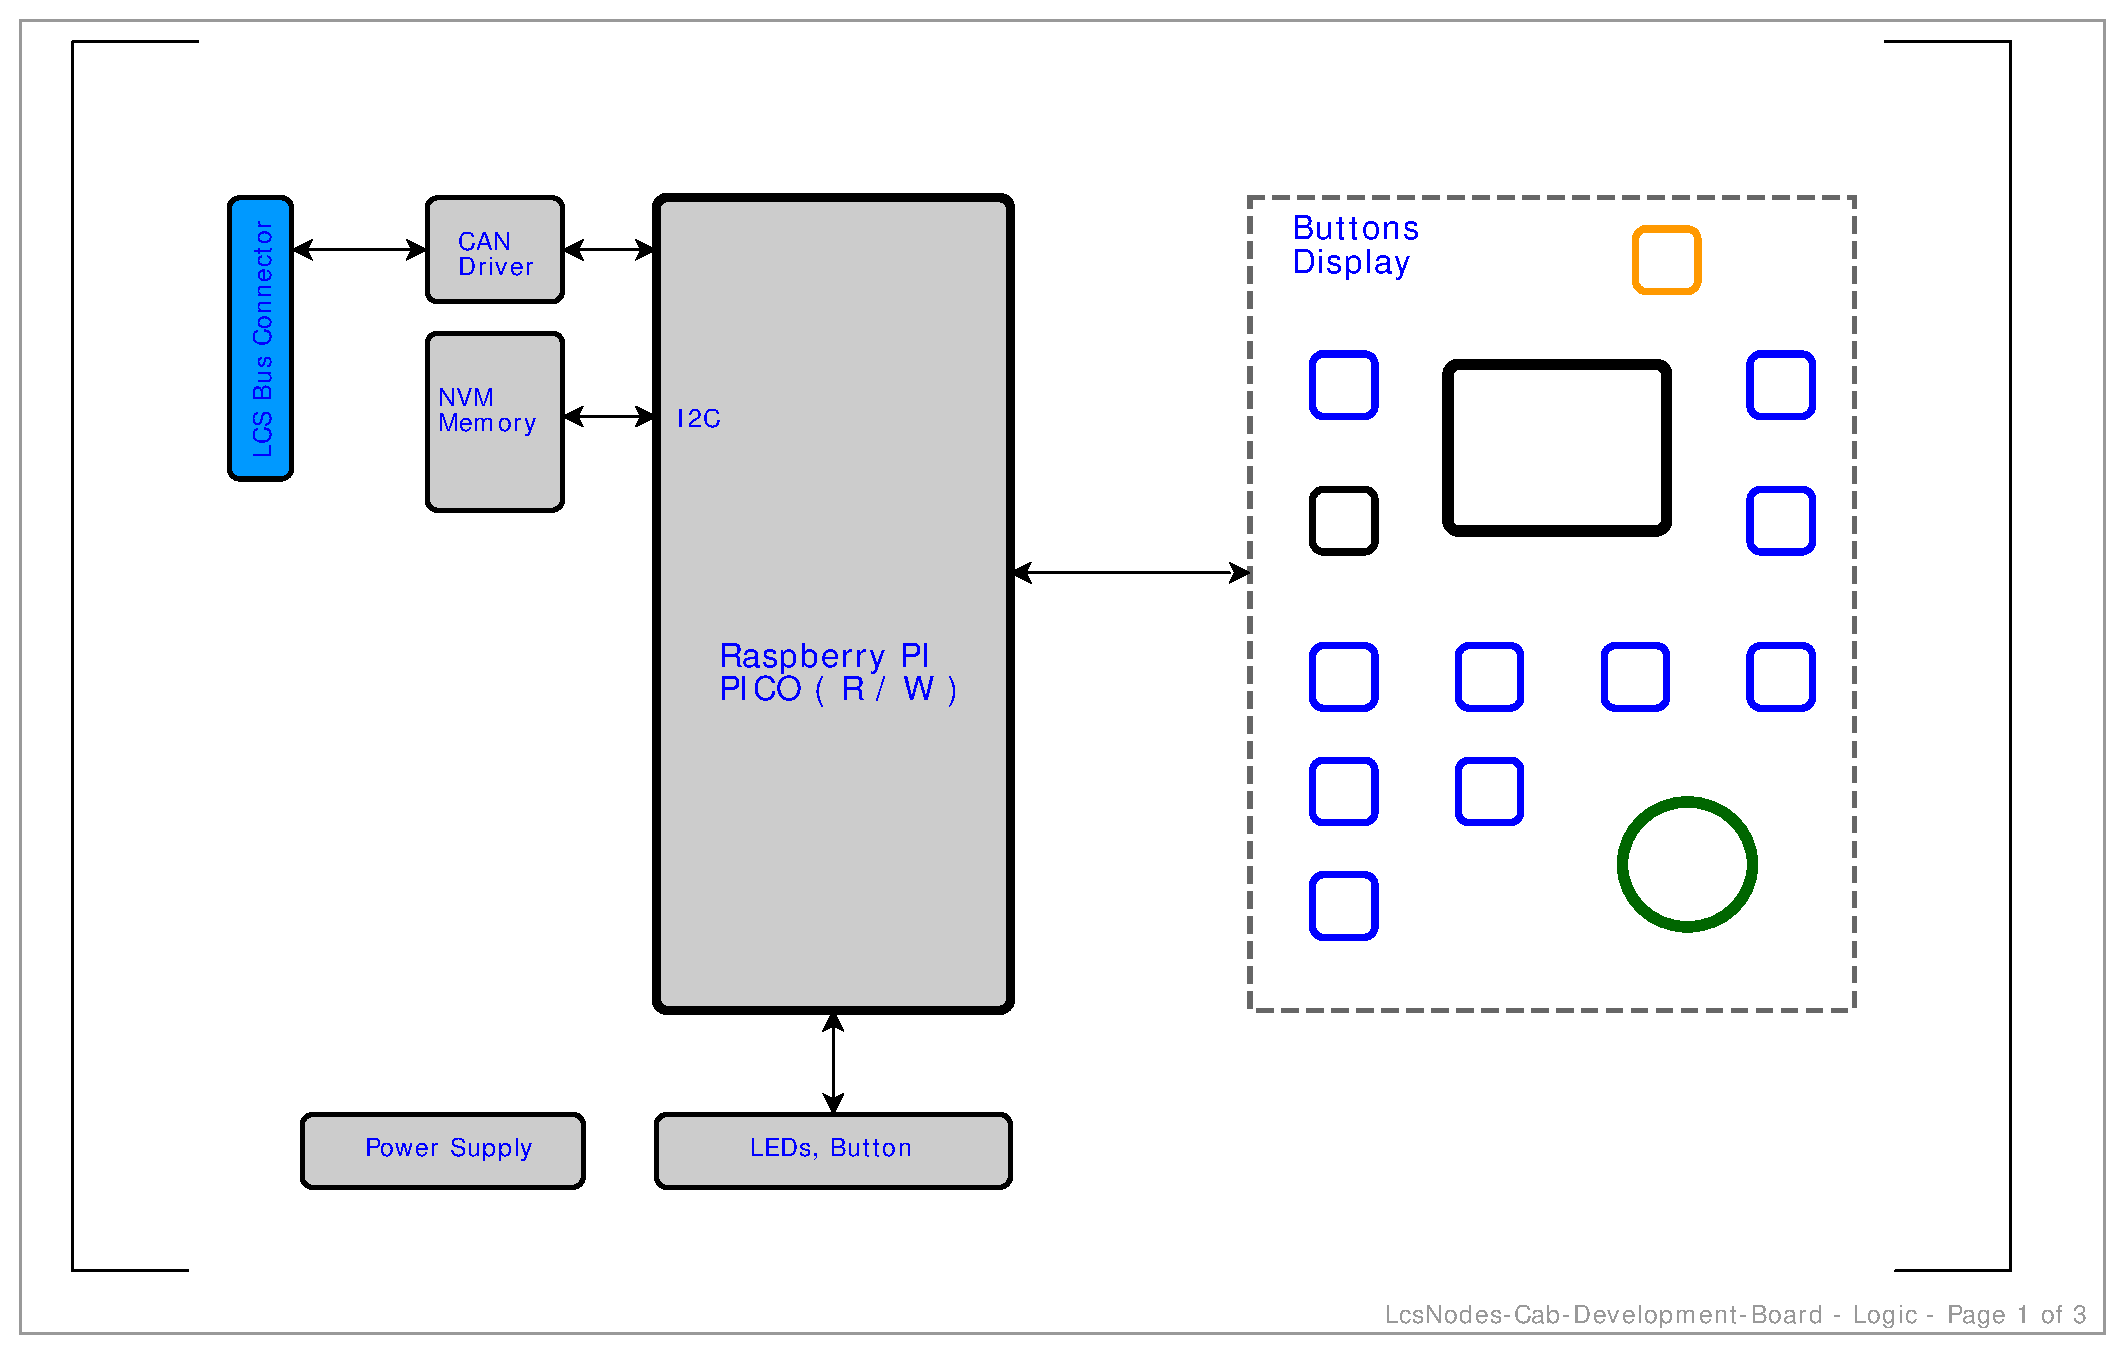
\includegraphics[page=1, width=0.9\textwidth]{./Schematics/Schematic_LcsNodes-Cab-Dev.pdf}
    \caption{Block Diagram}
    %\label{fig:schematic}
\end{figure}

There is essentially a main controller part with the Raspberry Pi Pico, a CAN bus interface and the non-volatile memory. This part should be very familiar by now. Besides the two I2C connections and the CAN bus pins, almost all GPIO pins are dedicated to a button or encoder. Since the GPIOs can be configured with internal pull-up, no external resistors are necessary. The power supply will be fed from the LCS bus. The whole board can also be fed from the USB port of the PICO. Again, this is very handy for initial debugging the firmware. The LCS Bus connector will connect the cab handheld to the LCS layout. We use only the CAN Bus lines and optional the power line input.

\begin{figure}[htbp]
    \centering
    \includegraphics[page=2, width=0.9\textwidth]{./Schematics/Schematic_LcsNodes-Cab-Dev.pdf}
    \caption{Controller}
    %\label{fig:schematic}
\end{figure}
\FloatBarrier

Finally, there is the part with all the buttons, encoders and the OLED Display. The following schematic completes the cap handheld schematic for firmware development.

\begin{figure}[htbp]
    \centering
    \includegraphics[page=3, width=0.9\textwidth]{./Schematics/Schematic_LcsNodes-Cab-Dev.pdf}
    \caption{UI Elements}
    %\label{fig:schematic}
\end{figure}
\FloatBarrier

Granted, it is not really a cab handheld to hold in your hands. Although the final version will have pretty much the same hardware ingredients, the form factor needs to be different. But for development, the setup will be quite helpful and robust. You will avoid chasing software problems that turn out to be just a loose connection on a breadboard. 

\section{A basic Cab Handheld}

As the name already suggests, the cab handheld is a handheld device with several buttons and a display. To keep it a compact design, we will use both sides of the PCB. The upper side contains the buttons, switches and display, the lower side contains the controller components. The cab handheld will connect via a cable to the LCS bus. Power comes from the LCS bus power lines and the CAN bus interface is used to transmit the messages. Perhaps a later version will also add some WLAN capabilities. While WLAN would come pretty much for free with the PICO W, the power supply side needs to include a battery.

\begin{itemize}
\item a 8x12cm board, used from both sides (?)
\item block diagram...
\item power supply from the LCS bus lines
\item controller, a PICO
\item small display
\item rotary encoder, switches, buttons, etc.
\item a subset for analog ?
\end{itemize}

// ??? \textbf{note} to do ..... focus on the firmware first ...

\section{Cab Handheld Firmware}

Now that the development platform is in place, let's have a look at the firmware design. As you perhaps have guessed it, the hardware was already developed with a certain mode in mind. First of all, a cab handheld is nothing else than just another node on the LCS bus. The firmware sits on top of the LCS core library. In addition, there is another key library we have not talked about yet. A cab handheld and also any other device that allows for users to interact, needs software to work with buttons, encoders, displays and so on. This the tasks of the \textbf{UI Elements } library. We will look at this library in a later chapter in great detail.

// ??? note perhaps a picture ?

\begin{itemize}
\item SW architecture on top of the LCS library
\item UI is key to build a handheld
\item firmware to handle the buttons, switches, display, etc. Refer to UIElements.
\item issues LCS messages to the base station for speed, direction and functions
\item menu descriptions
\end{itemize}

\subsection{Concepts}

\begin{itemize}
\item a current cab and a stack of cabs to select from
\item base station has the ultimate data about a cab, loaded into the cab handheld
\item CabHandheld functions and DCC functions
\end{itemize}

\subsection{Screen Layout}

\begin{itemize}
\item display has 4 lines up to 16 characters. Two fonts
\item four navigation buttons, use top and bottom line, 8x8 font
\item two data lines between, 8x16 font.
\end{itemize}

\subsection{Screen Navigation}

\begin{itemize}
\item inherent in the UI Elements Screen Object design
\item MENU
\item SELECT
\item UP
\item DOWN
\end{itemize}

\subsection{Operate Screen}

\begin{itemize}
\item main screen, workhorse
\item speed, dir, functions
\end{itemize}

\subsection{Engine On/off Screen}

\begin{itemize}
\item for diesels only
\end{itemize}

\subsection{Engine Lights Screen}

\begin{itemize}
\item front and back lights...
\end{itemize}

\subsection{New Cab Screen}

There needs to be a way to set an engine cab number. The NEW CAB screen is used to enter a cab Id and engine type. We will display 4 digits and the engine type among we can toggle with the MENU button. The UP/DOWN buttons advance the current digit position. The encoder knob offers a fast way to scroll a digit. The high value digit allows to set an "S" instead of the number to indicate a short loco DCC address. The SELECT button completes the number entering and the current cab becomes this new cab. Note, that it would need to be explicitly saved.

\begin{itemize}
\item works on current cab setting
\end{itemize}

\subsection{Select Cab Screen}

A cab handheld maintains a stack of known cabs. That is cabs the handheld has used before and saved in the cab stack. This menu will toggle through them and select the new current cab. The UP/DOWN button is used to scroll around. In addition, the encoder knob allows to scroll a bit faster. The SELECT button will make the entry shown the current loco.

\begin{itemize}
\item SELECT scrolls through the cab stack and sets the cab selected as current cab.
\end{itemize}

\subsection{Save Cab Screen}

The current cab can be saved in the cab stack. This menu will toggle through them and select the cab slot for saving the current cab data. The UP/DOWN button is used to scroll around. In addition, the encoder knob allows to scroll a bit faster. The SELECT button will perform the action.

\begin{itemize}
\item SAVE scrolls through the cab stack and saves the current cab to this slot.
\item any previous entry used for the same cabId is cleared.
\end{itemize}

\subsection{Set DCC Function}

The DCC standard defines a list of 69 functions, F0 to F68.

\begin{itemize}
\item allows to set any DCC function ( F0 to F68 )
\item encoder knob for fast scrolling
\end{itemize}

\subsection{Config Cab Handheld Functions}

\begin{itemize}
\item connects a cab handheld function to a DCC function
\end{itemize}

\subsection{Options}

\begin{itemize}
\item all kinds of screen for configuration settings
\end{itemize}

\subsection{Diag}

\begin{itemize}
\item all kinds of screen for technical checks and tests
\end{itemize}

\subsection{Summary}

Phew. The cab handheld is another big step toward in operating a layout. After all, a layout control system without some form cab handhelds is not very useful. As said, there are many ways to build a cab. The design of UI elements and firmware was greatly influenced by a handheld called \textbf{\textit{Protothrottle}}. The concept of the four screen menu control buttons found its way into the UI Elements library. In addition to the general cab handheld, a cab handheld tailored toward a specific class of engines would be a great addition to operating that engine. The next section will present a diesel cab handheld that resembles a diesel cab stand from the 1950s.

\section{The Diesel Cab Handheld}

The general handheld for controlling a locomotive is just one possible implementation. There is a company, Iowa Scale Engineering, that has built a handled called the \textbf{\textit{Protothrottle}}. This wireless handheld implements as the control elements the cab of a diesel engine. Wow. There is a lever for the diesel engine prime mover, a level for the direction and one for the brakes. You operate the engine with setting the prime mover notch, release the brakes and then the engine moves. When putting the prime mover to "idle", the engine just roll until you apply the brakes. In short, a much more realistic way to operate a diesel locomotive. 

The diesel cab handheld will leverage many of the design elements of the general cab handheld. There is a display surrounded by the four buttons MENU, SEL, UP and DOWN. The software configuration menus follow the same principles. There are the four function buttons, the horn and the bell. Where the layout differs is that there is no knob for the speed. Instead throttle and brake levers are available. Also, the direction is modeled as a lever instead of two buttons. The following figure shows a rough sketch of the diesel cab handheld.

\begin{center}
    \begin{tikzpicture}[scale=0.9, transform shape]
        
     	\draw[help lines, gray!50, dashed] (0,0) grid(9,14);
     	
     	\node[ tsRoundedRectangle, 
                minimum width=9cm,
                minimum height=14cm,
                text width=3cm,
                text centered,
                fill=white!50] (display) at (4.5,7);

       	\node[ tsRoundedRectangle, 
                minimum width=3.5cm,
                minimum height=3.5cm,
                text width=3cm,
                text centered,
                fill=gray!30] (display) at (4.5,9.5) {Display};
        
        \node[ tsRoundedRectangle, 
                minimum width=1cm,
                minimum height=1cm,
                text width=1cm,
                text centered,
                fill=red!50] (horn) at (6.5,12.5) {Horn};
        
        \node[ tsRoundedRectangle, 
                minimum width=1cm,
                minimum height=1cm,
                text width=1cm,
                text centered,
                fill=blue!20] (menu) at (1.5,10.5) {Men};
                
      	\node[ tsRoundedRectangle, 
                minimum width=1cm,
                minimum height=1cm,
                text width=1cm,
                text centered,
                fill=blue!20] (up) at (7.5,10.5) {Up};

     	\node[ tsRoundedRectangle, 
                minimum width=1cm,
                minimum height=1cm,
                text width=1cm,
                text centered,
                fill=blue!20] (sel) at (1.5,8.5) {Sel};
                
    	\node[ tsRoundedRectangle, 
                minimum width=1cm,
                minimum height=1cm,
                text width=1cm,
                text centered,
                fill=blue!20] (down) at (7.5,8.5) {Dn};
                
     	\node[ tsRoundedRectangle, 
                minimum width=1cm,
                minimum height=1cm,
                text width=1cm,
                text centered,
                fill=red!50] (f1) at (1.5,6) {F1};
                
      	\node[ tsRoundedRectangle, 
                minimum width=1cm,
                minimum height=1cm,
                text width=1cm,
                text centered,
                fill=red!50] (f2) at (3.5,6) {F2};
                
      	\node[ tsRoundedRectangle, 
                minimum width=1cm,
                minimum height=1cm,
                text width=1cm,
                text centered,
                fill=red!50] (f3) at (5.5,6) {F3};
                
     	\node[ tsRoundedRectangle, 
                minimum width=1cm,
                minimum height=1cm,
                text width=1cm,
                text centered,
                fill=red!50] (f4) at (7.5,6) {F4};
                
      	\node[ tsRoundedRectangle, 
                minimum width=6cm,
                minimum height=0.75cm,
                text width=1cm,
                text centered,
                fill=red!50] (throttle) at (5,4.5) {Throttle};
                
                
       	\node[ tsRoundedRectangle, 
                minimum width=2cm,
                minimum height=0.75cm,
                text width=1cm,
                text centered,
                fill=red!50] (dir) at (6,3) {Dir};
                
      	\node[ tsRoundedRectangle, 
                minimum width=3cm,
                minimum height=0.75cm,
                text width=1cm,
                text centered,
                fill=red!50] (brake) at (2.5,2.5) {Brake};
                
                
       	\node[ tsRoundedRectangle, 
                minimum width=1cm,
                minimum height=1cm,
                text width=1cm,
                text centered,
                fill=red!50] (Bell) at (1.5,1) {Bell};
                
    \end{tikzpicture}
\end{center}


Leveraging the cab handheld hardware from the previous chapter, the diesel cab handheld just differs in the levers for throttle, direction and brake instead of the speed knob. All else is fairly the same. Let's get started.

\subsection{Requirements}

\begin{itemize}
\item Very similar to the previous cab handheld 
\item instead of speed knob, it features throttle and brake.
\item all else is about the same...
\end{itemize}

\subsection{Module hardware}

\begin{itemize}
\item Leverage the generic cab handheld
\item Controller with CanBus interface
\item power supply from the LCS bus lines
\item small display
\item rotary encoder, buttons, etc.
\end{itemize}

\subsection{Module firmware}

\begin{itemize}
\item UI elements are key again, leverage many screen built before
\item new part is how throttle and brake interplay to run the engine
\end{itemize}


\section{Summary}

\begin{itemize}
\item now we have a generic cab handheld and a diesel cab handheld.
\item one could come up with a steam or electric engine handheld. 
\item the firmware already goes a long way to quickly realize further cab handhelds.
\item would we ever build a handheld with other non-engine functionality... who knows... not right now.
\item would we build a version that can be integrated into a |\"Stellwerk\" table ? perhaps... just a main controller and an cab UI Elements extension
\end{itemize}

As always, there are many options to build a cab handheld. Although this version connects via cable to the LCS Bus, a wireless version is not hard to build. Having more buttons or fewer buttons, having a set of numeric keypad style input, are all quite valid options. It is a matter of what is preferred. Currently, the cab handheld will not offer any controls for accessories, such as turnouts. This is a subject better left to the layout control panels and controlling software. Our cab handheld favors the approach to model more of a locomotive control stand rather than a TV remote style handheld. Since this is a matter of taste and preference, go build your own.

There is certainly the option to connect commercially available handhelds. This would require to provide a gateway from let's say a LocoNet protocol based handheld to the LCS protocol. Refer to the base station part where is shows an optional LocoNet interface. Well, one day you should be able to connect such handhelds via the LocoNet bus. But right now the topic is on the backlog list.